\chapter{Annex}
\label{cha:annex}
\section{Logbook}
\label{sec:logbook}

\begin{table}[!ht]
    \caption{Logbook}
    \label{tab:logbook}
    \setlength\extrarowheight{2pt} % for a bit of visual "breathing space"
    \begin{tabularx}{\textwidth}{|>{\hsize=.15\hsize}X|>{\hsize=.85\hsize}X|}
        \hline
        \textbf{Date} & \textbf{Works}                                                                                                                                                       \\
        \hline
        7/1 - 7/3     & Study of SERPENT and preparation of model's geometry                                                                                                                 \\
        \hline
        7/3 - 7/5     & Preparation of model's materials and excel files to calculate different atom densities.                                                                              \\
        \hline
        7/5 - 7/8     & Calculation of a simple assembly's burnup for testing, compilation of a version of SERPENT that could draw geometry to .png files.                                   \\
        \hline
        7/8 - 7/10    & Tracking of atom densities of control rods, preparation of MATLAB scripts to read atom densities.                                                                    \\
        \hline
        7/10 - 7/14   & Quantification of burnup of control rods using hot neutron flux in control rods. Study of the relation between $\Delta\Sigma^{cr}$ and $\int_{\mathcal{T}}\phi_hdt$. \\
        \hline
        7/14 - 7/17   & Quantification of burnup of control rods using formula of $B_{cr}$, deduction and calculation of $k$.                                                                \\
        \hline
        7/17 - 7/23   & Installation and study of TensorFlow.                                                                                                                                \\
        \hline
        7/23 - 8/4    & Quantification of burnup of control rods using assembly average neuron flux, regression of new $k$ and verification.                                                 \\
        \hline
        8/4 - 8/7     & Preparation of Python scripts of data acquisition.                                                                                                                   \\
        \hline
        8/7 - 8/19    & Several times of (data acquisition - train - evaluation) and analyzation of results.                                                                                 \\
        \hline
        8/19 - 8/21   & Preparation of report.                                                                                                                                               \\
        \hline
    \end{tabularx}
\end{table}

\newpage
\section{Amazement report}
\label{sec:amazement_report}

In this stage of two months, I find that the relation between colleagues in the office not as formal as I imagined.
I didn't notice any problem of corruption but still when there are some office-wide works (like fetching launch)
we avoid letting high level people do the work.
There are some institute-wide dinners where people should participate if they what to be sociable. However, I managed to avoid one.
I heard that in some governmental organizations this kind of dinners are inevitable and corruption is very serious.

I'm a little astonished that the canteen in the university is better than the canteen here.
Perhaps because of the epidemic, there are few choices and only very specific dishes can be eaten inside the canteen.

All the computers distributed by the enterprise could not connect to Internet, and it's very difficult to install softwares.
Same for the servers that I used to do the simulations.
Although I understand this is for the information security, it's still quite annoying the reduces the efficiency of coding.
In my case, many work are done in my laptop and copied to enterprise's computers.
(We cannot copy anything from enterprise's computers.)

If a student studies normally in IFCEN, he should be able to code with C++, Python and use Linux servers without any problems.
These capabilities are very important in many aspects of work because many jobs require direct application of these capacities.
In addition, a solid knowledge of physics (chemistry) is also very important.
It helps understand the problems quickly and propose various types of possibilities and solutions.
In this stage, the software used, SERPENT is very similar to the software we've studied in IFCEN TRIPOLI.
In fact, I see no other differences except grammar of input cards.
Monte Carlo simulation softwares are almost all like this and once you've learned how to use one of them, it's very easy to study others.



\newpage
\section{Reception service organization chart}
\label{sec:organization_chart}
\begin{figure}[!htb]
    \centering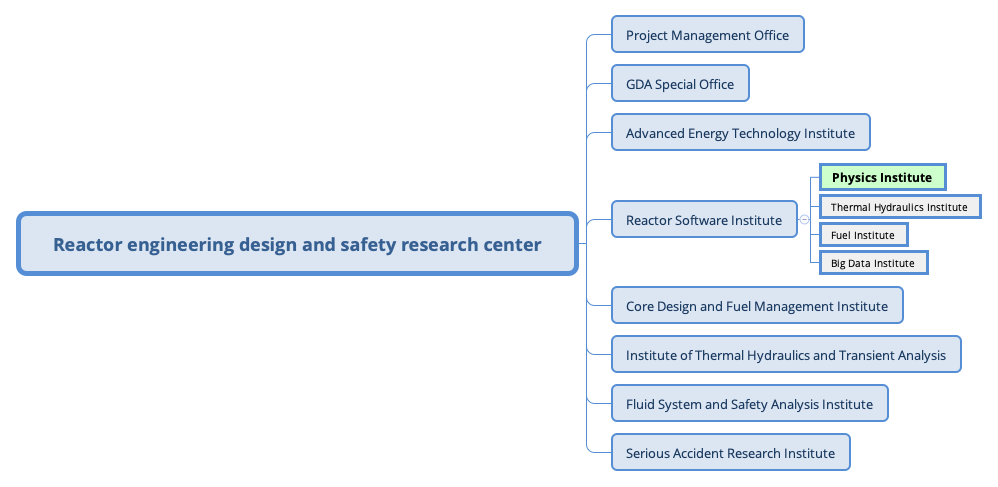
\includegraphics[width=1\linewidth]{Figs/Organigramme.png}
    \caption{Organization chart of reception service, the green block is where the stage took place.}
    \label{fig:organigramme}
\end{figure}